\documentclass{article}\usepackage[]{graphicx}\usepackage[]{color}
%% maxwidth is the original width if it is less than linewidth
%% otherwise use linewidth (to make sure the graphics do not exceed the margin)
\makeatletter
\def\maxwidth{ %
  \ifdim\Gin@nat@width>\linewidth
    \linewidth
  \else
    \Gin@nat@width
  \fi
}
\makeatother

\definecolor{fgcolor}{rgb}{0.345, 0.345, 0.345}
\newcommand{\hlnum}[1]{\textcolor[rgb]{0.686,0.059,0.569}{#1}}%
\newcommand{\hlstr}[1]{\textcolor[rgb]{0.192,0.494,0.8}{#1}}%
\newcommand{\hlcom}[1]{\textcolor[rgb]{0.678,0.584,0.686}{\textit{#1}}}%
\newcommand{\hlopt}[1]{\textcolor[rgb]{0,0,0}{#1}}%
\newcommand{\hlstd}[1]{\textcolor[rgb]{0.345,0.345,0.345}{#1}}%
\newcommand{\hlkwa}[1]{\textcolor[rgb]{0.161,0.373,0.58}{\textbf{#1}}}%
\newcommand{\hlkwb}[1]{\textcolor[rgb]{0.69,0.353,0.396}{#1}}%
\newcommand{\hlkwc}[1]{\textcolor[rgb]{0.333,0.667,0.333}{#1}}%
\newcommand{\hlkwd}[1]{\textcolor[rgb]{0.737,0.353,0.396}{\textbf{#1}}}%
\let\hlipl\hlkwb

\usepackage{framed}
\makeatletter
\newenvironment{kframe}{%
 \def\at@end@of@kframe{}%
 \ifinner\ifhmode%
  \def\at@end@of@kframe{\end{minipage}}%
  \begin{minipage}{\columnwidth}%
 \fi\fi%
 \def\FrameCommand##1{\hskip\@totalleftmargin \hskip-\fboxsep
 \colorbox{shadecolor}{##1}\hskip-\fboxsep
     % There is no \\@totalrightmargin, so:
     \hskip-\linewidth \hskip-\@totalleftmargin \hskip\columnwidth}%
 \MakeFramed {\advance\hsize-\width
   \@totalleftmargin\z@ \linewidth\hsize
   \@setminipage}}%
 {\par\unskip\endMakeFramed%
 \at@end@of@kframe}
\makeatother

\definecolor{shadecolor}{rgb}{.97, .97, .97}
\definecolor{messagecolor}{rgb}{0, 0, 0}
\definecolor{warningcolor}{rgb}{1, 0, 1}
\definecolor{errorcolor}{rgb}{1, 0, 0}
\newenvironment{knitrout}{}{} % an empty environment to be redefined in TeX

\usepackage{alltt}

% \usepackage[utf8]{inputenc}
\usepackage{amsmath}
\usepackage{fancyhdr}
\usepackage{array}
\usepackage{longtable}
\usepackage{graphicx}
\usepackage{color}
\usepackage[letterpaper, margin=1in]{geometry}
\usepackage{lscape}
\newcommand{\blandscape}{\begin{landscape}}
\newcommand{\elandscape}{\end{landscape}}
\usepackage{dcolumn}
\usepackage{bbm}
\usepackage{threeparttable}
\usepackage{booktabs}
\usepackage{expex}
\usepackage{pdflscape}
\usepackage{rotating, graphicx}
\usepackage{tabulary}
\usepackage{lscape}
\usepackage{makecell}
\usepackage{algorithm}
\usepackage{multirow}
\usepackage{colortbl}
\usepackage{longtable}
\usepackage{array}
\usepackage{multirow}
\usepackage{wrapfig}
\usepackage{float}
\usepackage{pdflscape}
\usepackage{tabu}
\usepackage{threeparttable}

\title{%
Homework 3\\
\large Applied Mutlivariate Analysis}
\date{September 22, 2018}
\author{Emorie Beck}
\IfFileExists{upquote.sty}{\usepackage{upquote}}{}
\begin{document}
\maketitle
% \SweaveOpts{concordance=TRUE}

\section{Workspace}
\subsection{Packages}



\begin{knitrout}
\definecolor{shadecolor}{rgb}{0.969, 0.969, 0.969}\color{fgcolor}\begin{kframe}
\begin{alltt}
\hlkwd{library}\hlstd{(car)}
\hlkwd{library}\hlstd{(knitr)}
\hlkwd{library}\hlstd{(psych)}
\hlkwd{library}\hlstd{(kableExtra)}
\hlkwd{library}\hlstd{(multcomp)}
\hlkwd{library}\hlstd{(lme4)}
\hlkwd{library}\hlstd{(plyr)}
\hlkwd{library}\hlstd{(tidyverse)}
\hlkwd{library}\hlstd{(MVN)}
\end{alltt}
\end{kframe}
\end{knitrout}

\subsection{data}
The file, Set\_3.csv, contains the data from a study in which 500 high school students completed a measure of scholastic aptitude: Grammar, Paragraph Comprehension, Vocabulary, Sentence Completion, Geometry, Algebra, Numerical Puzzles, Series Completion, Practical Problem Solving, Symbol Manipulation, Analytical Ability, and Formal Logic. 
\begin{knitrout}
\definecolor{shadecolor}{rgb}{0.969, 0.969, 0.969}\color{fgcolor}\begin{kframe}
\begin{alltt}
\hlstd{wd} \hlkwb{<-} \hlstr{"https://github.com/emoriebeck/homeworks/raw/master/multivariate/homeworks/homework3"}

\hlstd{dat} \hlkwb{<-} \hlkwd{sprintf}\hlstd{(}\hlstr{"%s/Set_3.csv"}\hlstd{, wd)} \hlopt
  \hlkwd{read.csv}\hlstd{(.,} \hlkwc{stringsAsFactors} \hlstd{= F)}

\hlkwd{head}\hlstd{(dat)}
\end{alltt}
\begin{verbatim}
##   ID    Grammar Paragraph_Comprehension Vocabulary Sentence_Completion
## 1  1  2.0298794               0.7009379  0.9224983           0.7783650
## 2  2  1.8460110               0.8176540  1.6230497           0.5595109
## 3  3 -0.5514456               0.1155194 -0.2451959           1.2206362
## 4  4 -1.3804105               0.2193181  0.5195521           0.3530657
## 5  5  0.4384477               1.5177577  0.4692875           1.4074032
## 6  6 -0.5984267              -0.8757810 -0.9889196          -1.4836151
##     Geometry      Algebra Numerical_Puzzles Series_Completion
## 1  0.7169340  0.649042462         0.1797594       0.521331792
## 2 -1.4336680  0.008714271        -0.2517458       0.000110179
## 3 -0.5504154 -0.776083508         0.8131658      -0.802679845
## 4  1.7218792  1.076026142         0.7711456      -0.381686114
## 5  0.7914582  1.541237112         0.4042484       0.825899485
## 6 -0.5157728 -0.441559349        -1.0049260      -2.612748945
##   Practical_Problem_Solving Symbol_Manipulation Analytical_Ability
## 1                 1.3030926           1.3690616          1.5512126
## 2                 0.9545397          -0.9592880          1.4883905
## 3                -1.5259042          -1.2038384         -0.7812775
## 4                -0.5231818           0.1203525         -0.3958278
## 5                 1.2598039           2.6013012          0.9772288
## 6                -0.1936980          -0.1956773         -0.2486582
##   Formal_Logic
## 1    0.7546186
## 2   -0.3733971
## 3   -1.1192996
## 4    1.7353933
## 5    3.0419200
## 6   -0.8137567
\end{verbatim}
\end{kframe}
\end{knitrout}

Answer the following questions about these data:

\section{Question 1}
What evidence do you have that these data should be subjected to a principal components analysis? 

\begin{knitrout}
\definecolor{shadecolor}{rgb}{0.969, 0.969, 0.969}\color{fgcolor}\begin{kframe}
\begin{alltt}
\hlstd{R} \hlkwb{<-} \hlstd{dat} \hlopt \hlkwd{select}\hlstd{(}\hlopt{-}\hlstd{ID)} \hlopt \hlstd{cor}

\hlstd{(KMO1} \hlkwb{<-} \hlkwd{KMO}\hlstd{(R))}
\end{alltt}
\begin{verbatim}
## Kaiser-Meyer-Olkin factor adequacy
## Call: KMO(r = R)
## Overall MSA =  0.82
## MSA for each item = 
##                   Grammar   Paragraph_Comprehension 
##                      0.83                      0.84 
##                Vocabulary       Sentence_Completion 
##                      0.83                      0.82 
##                  Geometry                   Algebra 
##                      0.82                      0.83 
##         Numerical_Puzzles         Series_Completion 
##                      0.77                      0.84 
## Practical_Problem_Solving       Symbol_Manipulation 
##                      0.84                      0.81 
##        Analytical_Ability              Formal_Logic 
##                      0.82                      0.83
\end{verbatim}
\begin{alltt}
\hlstd{(CB_1} \hlkwb{<-} \hlkwd{cortest.bartlett}\hlstd{(}\hlkwc{R}\hlstd{=R,}\hlkwc{n}\hlstd{=}\hlkwd{nrow}\hlstd{(dat)))}
\end{alltt}
\begin{verbatim}
## $chisq
## [1] 1794.866
## 
## $p.value
## [1] 0
## 
## $df
## [1] 66
\end{verbatim}
\end{kframe}
\end{knitrout}
The overall MSA is .82, and all but one of the MSA values are .8 (1 (Numerical Puzzles) is .77), which indicates very strong evidence for conducting a PCA.  

In addition, the $\chi^2$ value of the Bartlett test ($\chi^2$(66) = 1794.87), which indicates that the correlation matrix departs significantly from from an identity matrix (independence among indicators).  

\section{Question 2}
How many principal components should be extracted?
\begin{knitrout}
\definecolor{shadecolor}{rgb}{0.969, 0.969, 0.969}\color{fgcolor}\begin{kframe}
\begin{alltt}
\hlkwd{par}\hlstd{(}\hlkwc{mfrow}\hlstd{=}\hlkwd{c}\hlstd{(}\hlnum{1}\hlstd{,}\hlnum{2}\hlstd{))}
\hlstd{scree_1} \hlkwb{<-} \hlkwd{fa.parallel}\hlstd{(dat} \hlopt \hlkwd{select}\hlstd{(}\hlopt{-}\hlstd{ID),} \hlkwc{fa}\hlstd{=}\hlstr{"pc"}\hlstd{)}
\end{alltt}
\begin{verbatim}
## Parallel analysis suggests that the number of factors =  NA  and the number of components =  3
\end{verbatim}
\begin{alltt}
\hlstd{scree_2} \hlkwb{<-} \hlkwd{fa.parallel}\hlstd{(R,} \hlkwc{fa} \hlstd{=} \hlstr{"pc"}\hlstd{,} \hlkwc{n.obs} \hlstd{=} \hlkwd{nrow}\hlstd{(dat))}
\end{alltt}
\end{kframe}
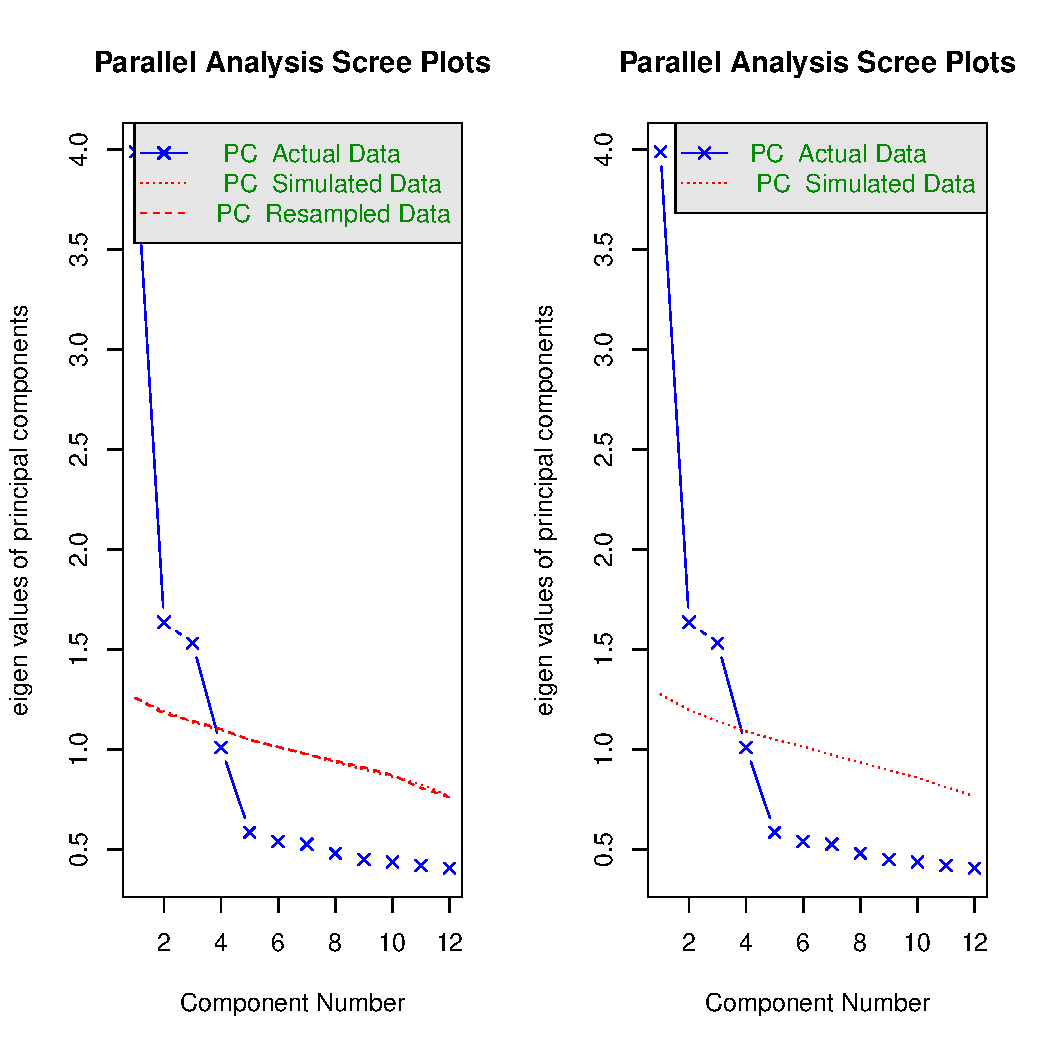
\includegraphics[width=\maxwidth]{figure/unnamed-chunk-5-1} 
\begin{kframe}\begin{verbatim}
## Parallel analysis suggests that the number of factors =  NA  and the number of components =  3
\end{verbatim}
\end{kframe}
\end{knitrout}

Parallel analysis suggests that 3 factors should be extracted from the data. 

\section{Question 3}
How much variance do these extracted components account for in the original data?
\begin{knitrout}
\definecolor{shadecolor}{rgb}{0.969, 0.969, 0.969}\color{fgcolor}\begin{kframe}
\begin{alltt}
\hlstd{pca_1} \hlkwb{<-} \hlkwd{principal}\hlstd{(R,} \hlkwc{nfactors} \hlstd{=} \hlnum{3}\hlstd{,} \hlkwc{rotate} \hlstd{=} \hlstr{"none"}\hlstd{,} \hlkwc{n.obs} \hlstd{=} \hlkwd{nrow}\hlstd{(dat),} \hlkwc{residuals} \hlstd{= T)}

\hlstd{pca_1}\hlopt{$}\hlstd{Vaccounted} \hlopt \hlstd{data.frame} \hlopt \hlkwd{mutate}\hlstd{(}\hlkwc{m} \hlstd{=} \hlkwd{rownames}\hlstd{(.))} \hlopt
  \hlkwd{mutate_at}\hlstd{(}\hlkwd{vars}\hlstd{(PC1}\hlopt{:}\hlstd{PC3),} \hlkwd{funs}\hlstd{(}\hlkwd{round}\hlstd{(.,}\hlnum{2}\hlstd{)))} \hlopt
  \hlkwd{select}\hlstd{(m,} \hlkwd{everything}\hlstd{())} \hlopt
  \hlkwd{kable}\hlstd{(.,} \hlstr{"latex"}\hlstd{,} \hlkwc{booktabs} \hlstd{= T,} \hlkwc{escape} \hlstd{= F)}
\end{alltt}
\end{kframe}
\begin{tabular}{lrrr}
\toprule
m & PC1 & PC2 & PC3\\
\midrule
SS loadings & 3.99 & 1.64 & 1.53\\
Proportion Var & 0.33 & 0.14 & 0.13\\
Cumulative Var & 0.33 & 0.47 & 0.60\\
Proportion Explained & 0.56 & 0.23 & 0.21\\
Cumulative Proportion & 0.56 & 0.79 & 1.00\\
\bottomrule
\end{tabular}


\end{knitrout}

The three extracted components account for all of the variance. 

\section{Question 4}
How much variance in the original Geometry variable is accounted for by these extracted components?  
The extracted components account for 57.85\% of the variance in the original Geometry variable.  


\section{Question 5}
Now screen the data for unusual cases and determine if your conclusions change when
any such cases are excluded from the analysis.  

If you believe there is more than one outlier in the data, follow a sequential approach to determining how many to exclude. This means that you will identify the worst offender, exclude that case, and then repeat your diagnostics to determine if other outliers are present. If so, again exclude the worst one, and repeat the diagnostics to determine if an additional outlier is present. Keep cycling through these steps until you are satisfied you have all outliers identified and excluded. Then conduct the principal components analysis. This iterative approach is necessary for multivariate diagnostics such as Mahalanobis distance because the presence of one outlier can influence the apparent presence of others via their joint influence on the covariance matrix. Removing them one at a time insures you don’t miss any or mistakenly remove cases that are not really outliers.  

\begin{knitrout}
\definecolor{shadecolor}{rgb}{0.969, 0.969, 0.969}\color{fgcolor}\begin{kframe}
\begin{alltt}
\hlstd{dat} \hlopt
  \hlkwd{gather}\hlstd{(indicator, value,} \hlopt{-}\hlstd{ID)} \hlopt
  \hlkwd{ggplot}\hlstd{(}\hlkwd{aes}\hlstd{(}\hlkwc{x} \hlstd{= indicator,} \hlkwc{y} \hlstd{= value,} \hlkwc{fill} \hlstd{= indicator))} \hlopt{+}
    \hlkwd{geom_boxplot}\hlstd{()} \hlopt{+}
    \hlkwd{coord_flip}\hlstd{()} \hlopt{+}
    \hlkwd{theme_classic}\hlstd{()} \hlopt{+}
    \hlkwd{theme}\hlstd{(}\hlkwc{legend.position} \hlstd{=} \hlstr{"none"}\hlstd{)}
\end{alltt}
\end{kframe}
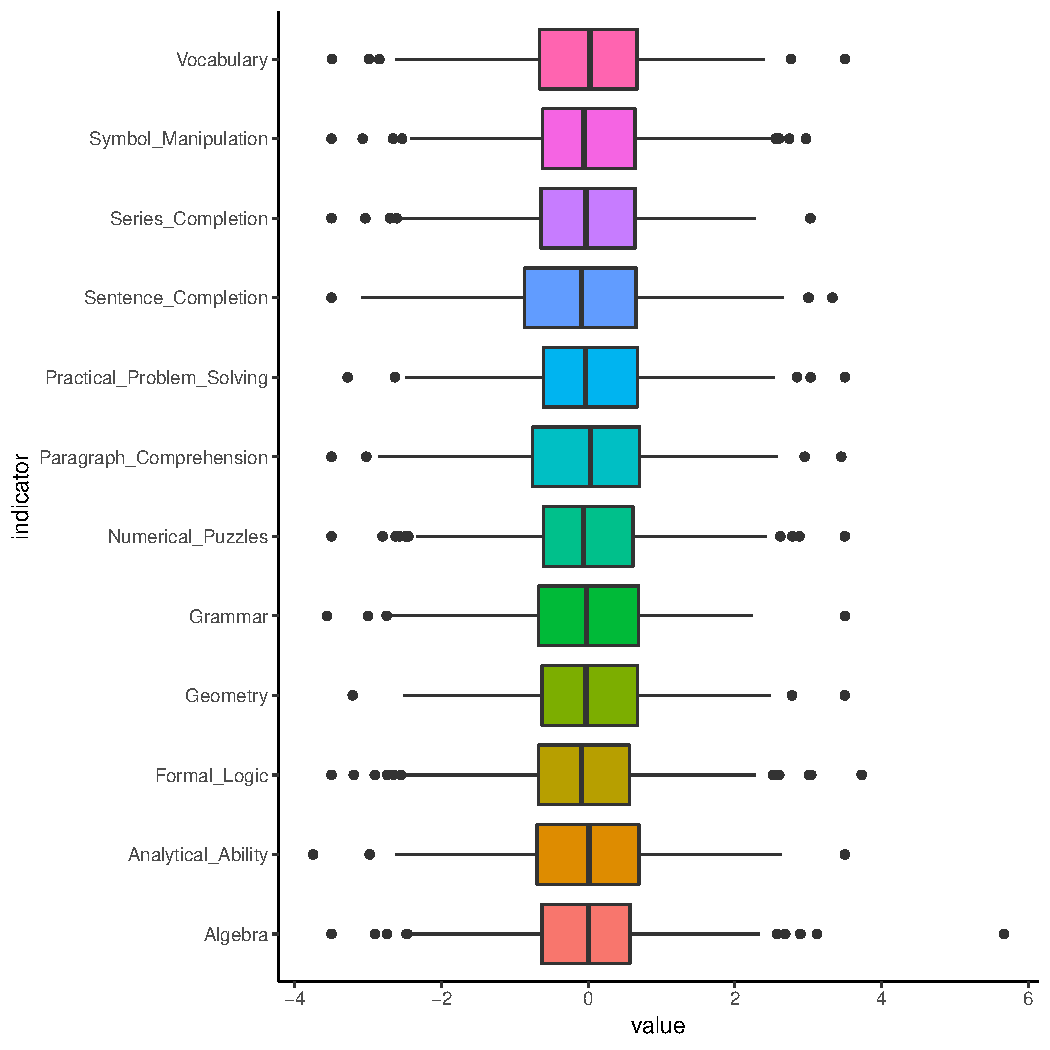
\includegraphics[width=\maxwidth]{figure/unnamed-chunk-7-1} 

\end{knitrout}

Visual inspection of the boxplot suggests there is one outlier in the algebra indicator, but let's check multivariate normality before making a decision.

\begin{knitrout}
\definecolor{shadecolor}{rgb}{0.969, 0.969, 0.969}\color{fgcolor}\begin{kframe}
\begin{alltt}
\hlstd{(pca_2} \hlkwb{<-} \hlkwd{principal}\hlstd{(}
    \hlstd{dat} \hlopt \hlkwd{select}\hlstd{(}\hlopt{-}\hlstd{ID)}
  \hlstd{,} \hlkwc{nfactors} \hlstd{=} \hlkwd{ncol}\hlstd{(dat)}\hlopt{-}\hlnum{1}
  \hlstd{,} \hlkwc{rotate} \hlstd{=} \hlstr{"none"}
  \hlstd{,} \hlkwc{residuals} \hlstd{= T}
  \hlstd{,} \hlkwc{scores} \hlstd{=} \hlnum{TRUE}\hlstd{)}
 \hlstd{)}
\end{alltt}
\begin{verbatim}
## Principal Components Analysis
## Call: principal(r = dat %>% select(-ID), nfactors = ncol(dat) - 1, 
##     residuals = T, rotate = "none", scores = TRUE)
## Standardized loadings (pattern matrix) based upon correlation matrix
##                            PC1   PC2   PC3   PC4   PC5   PC6   PC7   PC8
## Grammar                   0.62 -0.16 -0.46  0.27  0.04 -0.07  0.32 -0.20
## Paragraph_Comprehension   0.61 -0.09 -0.48 -0.30 -0.01 -0.24 -0.10  0.17
## Vocabulary                0.60 -0.18 -0.44  0.30 -0.25  0.36 -0.05 -0.04
## Sentence_Completion       0.60 -0.14 -0.50 -0.27  0.21 -0.04 -0.14  0.02
## Geometry                  0.51  0.55  0.09  0.23  0.39  0.34 -0.23  0.02
## Algebra                   0.56  0.46  0.10 -0.38 -0.21  0.19  0.27  0.34
## Numerical_Puzzles         0.48  0.60  0.09  0.32  0.11 -0.37  0.13  0.11
## Series_Completion         0.57  0.50  0.17 -0.20 -0.32 -0.08 -0.13 -0.46
## Practical_Problem_Solving 0.59 -0.31  0.34  0.30 -0.31 -0.09 -0.31  0.24
## Symbol_Manipulation       0.55 -0.35  0.44 -0.28  0.10  0.18  0.25 -0.08
## Analytical_Ability        0.60 -0.32  0.38  0.32  0.07 -0.07  0.20  0.00
## Formal_Logic              0.61 -0.33  0.37 -0.26  0.22 -0.09 -0.18 -0.09
##                             PC9  PC10  PC11  PC12 h2       u2 com
## Grammar                   -0.08  0.14 -0.04 -0.36  1 -1.3e-15 4.4
## Paragraph_Comprehension    0.22 -0.37 -0.14 -0.09  1  3.3e-16 4.5
## Vocabulary                 0.07  0.04 -0.20  0.29  1  1.2e-15 4.9
## Sentence_Completion       -0.14  0.18  0.38  0.18  1  1.3e-15 4.5
## Geometry                   0.05 -0.12  0.02 -0.17  1 -4.4e-16 4.8
## Algebra                   -0.22  0.05 -0.03 -0.05  1  4.4e-16 5.4
## Numerical_Puzzles          0.18  0.19 -0.07  0.22  1 -4.4e-16 4.6
## Series_Completion         -0.02 -0.08  0.09  0.00  1  1.1e-16 4.4
## Practical_Problem_Solving  0.05  0.14  0.15 -0.20  1 -2.2e-16 5.6
## Symbol_Manipulation        0.42  0.07  0.11  0.01  1 -2.2e-16 5.4
## Analytical_Ability        -0.25 -0.37  0.13  0.17  1 -2.2e-16 5.1
## Formal_Logic              -0.21  0.17 -0.38  0.03  1  4.4e-16 5.0
## 
##                        PC1  PC2  PC3  PC4  PC5  PC6  PC7  PC8  PC9 PC10
## SS loadings           3.99 1.64 1.53 1.01 0.58 0.54 0.52 0.48 0.45 0.44
## Proportion Var        0.33 0.14 0.13 0.08 0.05 0.04 0.04 0.04 0.04 0.04
## Cumulative Var        0.33 0.47 0.60 0.68 0.73 0.77 0.82 0.86 0.89 0.93
## Proportion Explained  0.33 0.14 0.13 0.08 0.05 0.04 0.04 0.04 0.04 0.04
## Cumulative Proportion 0.33 0.47 0.60 0.68 0.73 0.77 0.82 0.86 0.89 0.93
##                       PC11 PC12
## SS loadings           0.42 0.40
## Proportion Var        0.03 0.03
## Cumulative Var        0.97 1.00
## Proportion Explained  0.03 0.03
## Cumulative Proportion 0.97 1.00
## 
## Mean item complexity =  4.9
## Test of the hypothesis that 12 components are sufficient.
## 
## The root mean square of the residuals (RMSR) is  0 
##  with the empirical chi square  0  with prob <  NA 
## 
## Fit based upon off diagonal values = 1
\end{verbatim}
\begin{alltt}
\hlstd{scores_2} \hlkwb{<-} \hlstd{pca_2}\hlopt{$}\hlstd{scores} \hlopt \hlstd{data.frame}

\hlkwd{describe}\hlstd{(scores_2)}
\end{alltt}
\begin{verbatim}
##      vars   n mean sd median trimmed  mad    min   max range  skew
## PC1     1 500    0  1   0.01    0.01 0.97  -3.03  2.72  5.75 -0.12
## PC2     2 500    0  1   0.00   -0.02 1.02  -2.93  3.00  5.93  0.15
## PC3     3 500    0  1   0.03   -0.01 0.97  -3.06  3.10  6.16  0.06
## PC4     4 500    0  1  -0.04   -0.01 0.67 -10.78 11.72 22.50  0.71
## PC5     5 500    0  1   0.02    0.00 1.01  -4.09  2.68  6.77 -0.11
## PC6     6 500    0  1   0.00    0.02 0.96  -2.74  3.11  5.85 -0.14
## PC7     7 500    0  1   0.05    0.03 0.96  -3.22  3.17  6.39 -0.31
## PC8     8 500    0  1  -0.04   -0.01 0.98  -2.54  3.59  6.13  0.13
## PC9     9 500    0  1   0.02   -0.01 1.07  -3.21  3.10  6.31  0.03
## PC10   10 500    0  1  -0.03    0.00 0.94  -3.44  3.34  6.77  0.04
## PC11   11 500    0  1   0.03    0.02 0.98  -3.00  3.33  6.33 -0.08
## PC12   12 500    0  1   0.01    0.01 1.00  -2.67  2.90  5.56 -0.03
##      kurtosis   se
## PC1     -0.26 0.04
## PC2      0.01 0.04
## PC3      0.14 0.04
## PC4     62.60 0.04
## PC5      0.17 0.04
## PC6     -0.04 0.04
## PC7      0.10 0.04
## PC8      0.06 0.04
## PC9     -0.17 0.04
## PC10     0.27 0.04
## PC11     0.09 0.04
## PC12    -0.20 0.04
\end{verbatim}
\end{kframe}
\end{knitrout}

Checking the PCA suggests that there is a multivariate outlier in PCA 4 (Sentence\_Completion)

But let's check multivariate normality
\begin{knitrout}
\definecolor{shadecolor}{rgb}{0.969, 0.969, 0.969}\color{fgcolor}\begin{kframe}
\begin{alltt}
\hlstd{dat2} \hlkwb{<-} \hlstd{dat} \hlopt \hlkwd{select}\hlstd{(}\hlopt{-}\hlstd{ID)} \hlopt \hlstd{data.frame}
\hlkwd{rownames}\hlstd{(dat2)} \hlkwb{<-} \hlnum{1}\hlopt{:}\hlkwd{nrow}\hlstd{(dat2)}
\hlstd{(mv} \hlkwb{<-} \hlkwd{mvn}\hlstd{(dat2,}\hlkwc{mvnTest}\hlstd{=}\hlstr{"mardia"}\hlstd{,} \hlkwc{multivariatePlot}\hlstd{=}\hlstr{"qq"}\hlstd{,}\hlkwc{multivariateOutlierMethod}\hlstd{=}\hlstr{"quan"}\hlstd{,}\hlkwc{showOutliers}\hlstd{=}\hlnum{TRUE}\hlstd{))}
\end{alltt}
\end{kframe}
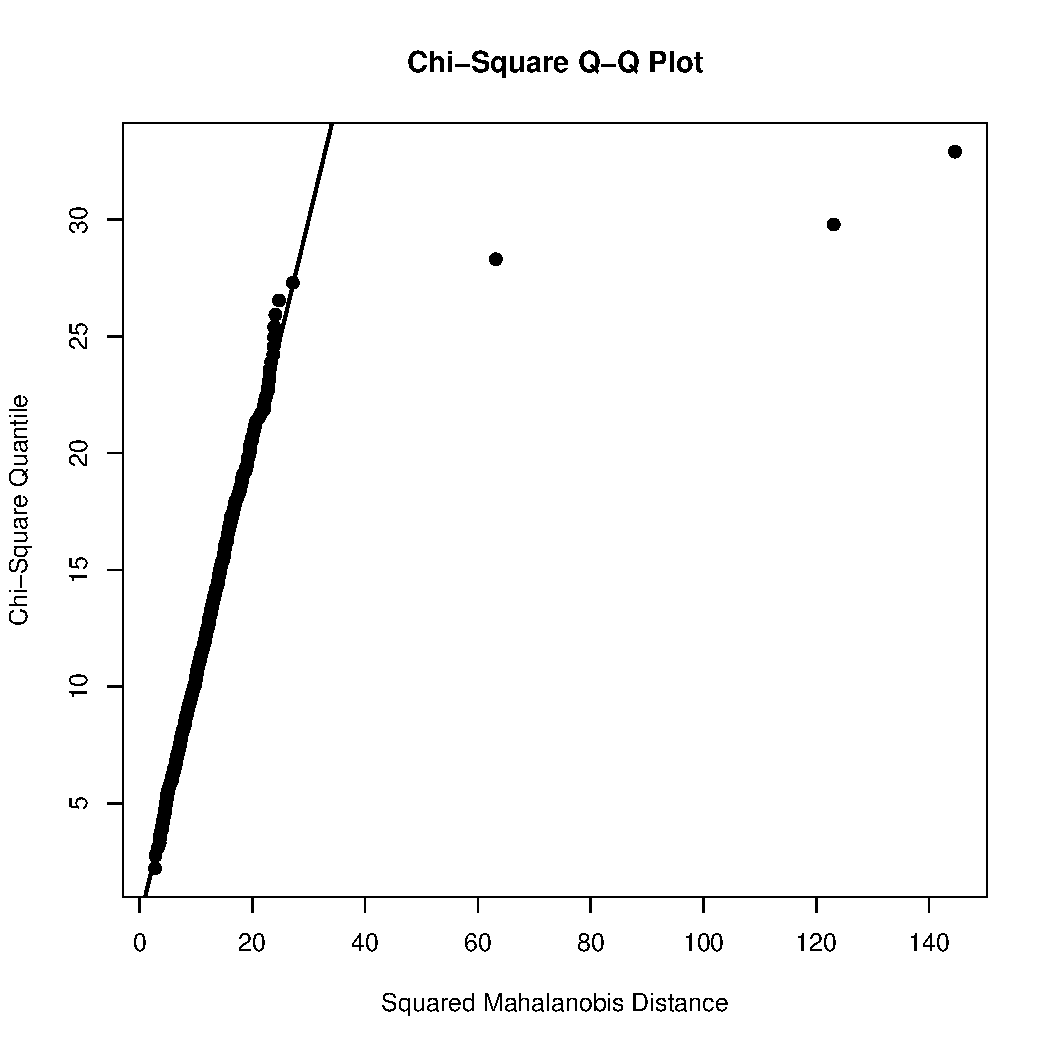
\includegraphics[width=\maxwidth]{figure/unnamed-chunk-9-1} 

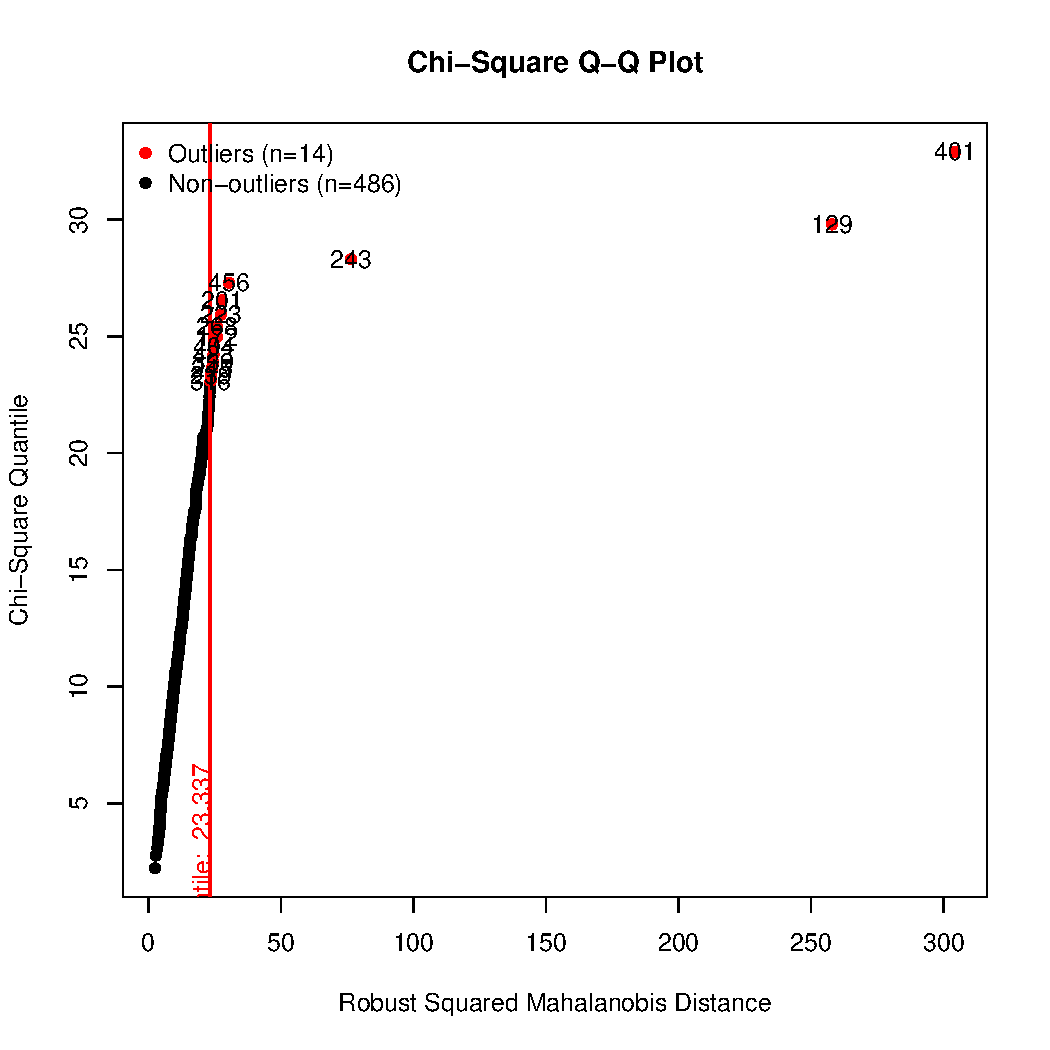
\includegraphics[width=\maxwidth]{figure/unnamed-chunk-9-2} 
\begin{kframe}\begin{verbatim}
## $multivariateNormality
##              Test        Statistic              p value Result
## 1 Mardia Skewness  468.99164354467 0.000162906731930752     NO
## 2 Mardia Kurtosis 37.8554992977048                    0     NO
## 3             MVN             <NA>                 <NA>     NO
## 
## $univariateNormality
##            Test                  Variable Statistic   p value Normality
## 1  Shapiro-Wilk          Grammar             0.9967  0.4074      YES   
## 2  Shapiro-Wilk  Paragraph_Comprehension     0.9989  0.9922      YES   
## 3  Shapiro-Wilk        Vocabulary            0.9958  0.1996      YES   
## 4  Shapiro-Wilk    Sentence_Completion       0.9981  0.8464      YES   
## 5  Shapiro-Wilk         Geometry             0.9978  0.7646      YES   
## 6  Shapiro-Wilk          Algebra             0.9835  <0.001      NO    
## 7  Shapiro-Wilk     Numerical_Puzzles        0.9968  0.4251      YES   
## 8  Shapiro-Wilk     Series_Completion        0.9971  0.5203      YES   
## 9  Shapiro-Wilk Practical_Problem_Solving    0.9967  0.4047      YES   
## 10 Shapiro-Wilk    Symbol_Manipulation       0.9956  0.1713      YES   
## 11 Shapiro-Wilk    Analytical_Ability        0.9977  0.7187      YES   
## 12 Shapiro-Wilk       Formal_Logic           0.9952  0.1221      YES   
## 
## $Descriptives
##                             n          Mean   Std.Dev        Median
## Grammar                   500 -0.0083641562 1.0016648 -0.0237048215
## Paragraph_Comprehension   500 -0.0070088967 1.0829739  0.0350785195
## Vocabulary                500 -0.0169538702 1.0169743  0.0232942325
## Sentence_Completion       500 -0.0903289108 1.1065777 -0.0893020655
## Geometry                  500  0.0071552259 0.9973637 -0.0282354790
## Algebra                   500 -0.0151778962 1.0149132  0.0003852515
## Numerical_Puzzles         500 -0.0153611723 1.0132508 -0.0624955155
## Series_Completion         500 -0.0077428597 0.9819436 -0.0291777090
## Practical_Problem_Solving 500 -0.0182512446 0.9584017 -0.0400207855
## Symbol_Manipulation       500 -0.0009142506 0.9922338 -0.0569430780
## Analytical_Ability        500 -0.0073984716 1.0009061  0.0090736190
## Formal_Logic              500 -0.0650934689 1.0367206 -0.0925315375
##                                 Min      Max       25th      75th
## Grammar                   -3.560000 3.500000 -0.6789687 0.6903545
## Paragraph_Comprehension   -3.500000 3.450000 -0.7551515 0.7002892
## Vocabulary                -3.491518 3.500000 -0.6651436 0.6660205
## Sentence_Completion       -3.500000 3.330000 -0.8637548 0.6525117
## Geometry                  -3.210000 3.500000 -0.6294255 0.6737671
## Algebra                   -3.500000 5.670000 -0.6288277 0.5685107
## Numerical_Puzzles         -3.500000 3.500000 -0.6082066 0.6101796
## Series_Completion         -3.500000 3.030000 -0.6444230 0.6380559
## Practical_Problem_Solving -3.280000 3.500000 -0.6115184 0.6685177
## Symbol_Manipulation       -3.500000 2.970000 -0.6179801 0.6397075
## Analytical_Ability        -3.751222 3.500000 -0.6981759 0.6938528
## Formal_Logic              -3.500000 3.728522 -0.6802409 0.5589411
##                                  Skew    Kurtosis
## Grammar                   -0.05430769  0.13596613
## Paragraph_Comprehension   -0.08800734  0.02507948
## Vocabulary                -0.20788125  0.16156136
## Sentence_Completion        0.02093275 -0.07335932
## Geometry                   0.11181433  0.10313111
## Algebra                    0.23409531  1.98559538
## Numerical_Puzzles          0.01651535  0.33457069
## Series_Completion         -0.13807654  0.07180595
## Practical_Problem_Solving  0.13693839  0.33690319
## Symbol_Manipulation        0.05168770  0.34049898
## Analytical_Ability        -0.11832265  0.22344750
## Formal_Logic               0.03731202  0.57661676
## 
## $multivariateOutliers
##     Observation Mahalanobis Distance Outlier
## 401         401              304.270    TRUE
## 129         129              257.852    TRUE
## 243         243               76.443    TRUE
## 456         456               30.479    TRUE
## 201         201               27.725    TRUE
## 223         223               27.365    TRUE
## 268         268               25.908    TRUE
## 172         172               25.869    TRUE
## 404         404               24.663    TRUE
## 423         423               24.565    TRUE
## 339         339               24.532    TRUE
## 245         245               23.903    TRUE
## 239         239               23.587    TRUE
## 316         316               23.477    TRUE
\end{verbatim}
\end{kframe}
\end{knitrout}

Based on the test of multivariate normality, there are 16(!) outliers. Let's remove the outlier and check again.

I'm going to use a while loop to do this rather than copying and pasting the code. 

\begin{knitrout}
\definecolor{shadecolor}{rgb}{0.969, 0.969, 0.969}\color{fgcolor}\begin{kframe}
\begin{alltt}
\hlstd{k} \hlkwb{<-} \hlnum{1}
\hlstd{remove} \hlkwb{<-} \hlkwd{c}\hlstd{()}
\hlkwd{par}\hlstd{(}\hlkwc{mfrow} \hlstd{=} \hlkwd{c}\hlstd{(}\hlnum{1}\hlstd{,}\hlnum{2}\hlstd{))}
\hlkwa{while}\hlstd{(}\hlkwd{nrow}\hlstd{(mv}\hlopt{$}\hlstd{multivariateOutliers)} \hlopt{>} \hlnum{0}\hlstd{)\{}
  \hlkwa{if}\hlstd{(k}\hlopt{!=}\hlnum{1}\hlstd{)\{tmp} \hlkwb{<-} \hlstd{dat2[}\hlopt{-}\hlstd{remove,]\}} \hlkwa{else}\hlstd{\{tmp} \hlkwb{<-} \hlstd{dat2\}}
  \hlstd{mv} \hlkwb{<-} \hlkwd{mvn}\hlstd{(tmp,} \hlkwc{mvnTest}\hlstd{=}\hlstr{"mardia"}\hlstd{,} \hlkwc{multivariatePlot}\hlstd{=}\hlstr{"none"}\hlstd{,}\hlkwc{multivariateOutlierMethod}\hlstd{=}\hlstr{"quan"}\hlstd{,}\hlkwc{showOutliers}\hlstd{=}\hlnum{TRUE}\hlstd{,} \hlkwc{univariatePlot} \hlstd{=} \hlstr{"none"}\hlstd{)}
  \hlstd{mv}\hlopt{$}\hlstd{multivariateOutliers}
  \hlstd{remove} \hlkwb{<-} \hlkwd{c}\hlstd{(remove,} \hlkwd{as.numeric}\hlstd{(}\hlkwd{as.character}\hlstd{(mv}\hlopt{$}\hlstd{multivariateOutliers}\hlopt{$}\hlstd{Observation[}\hlnum{1}\hlstd{])))}
  \hlkwd{sink}\hlstd{(}\hlstr{"/dev/null"}\hlstd{)}
  \hlstd{scree} \hlkwb{<-} \hlkwd{fa.parallel}\hlstd{(tmp,} \hlkwc{fa}\hlstd{=}\hlstr{"pc"}\hlstd{)}
  \hlkwd{sink}\hlstd{()}
  \hlkwd{print}\hlstd{(}\hlkwd{sprintf}\hlstd{(}\hlstr{"Case %s removed. %s factors remain. This is the %s round"}\hlstd{, remove[k], scree}\hlopt{$}\hlstd{ncomp, k))}
  \hlkwa{if}\hlstd{(}\hlkwd{nrow}\hlstd{(mv}\hlopt{$}\hlstd{multivariateOutliers)} \hlopt{==} \hlnum{0}\hlstd{)\{}\hlkwa{break}\hlstd{\}}
  \hlstd{k} \hlkwb{<-} \hlstd{k} \hlopt{+} \hlnum{1}
\hlstd{\}}
\end{alltt}
\end{kframe}
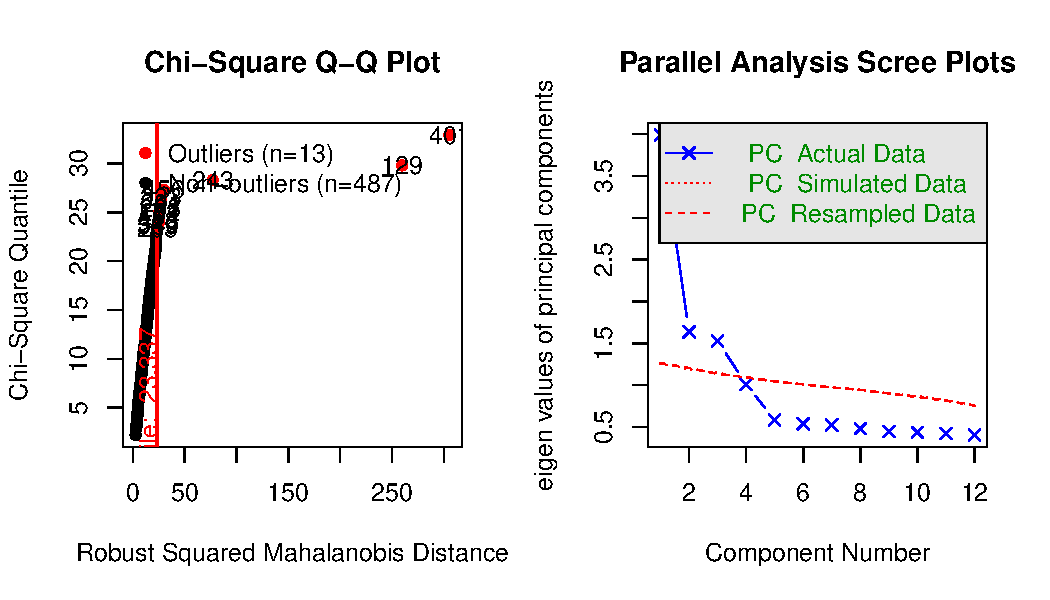
\includegraphics[width=\maxwidth]{figure/unnamed-chunk-10-1} 
\begin{kframe}\begin{verbatim}
## [1] "Case 401 removed. 3 factors remain. This is the 1 round"
\end{verbatim}
\end{kframe}
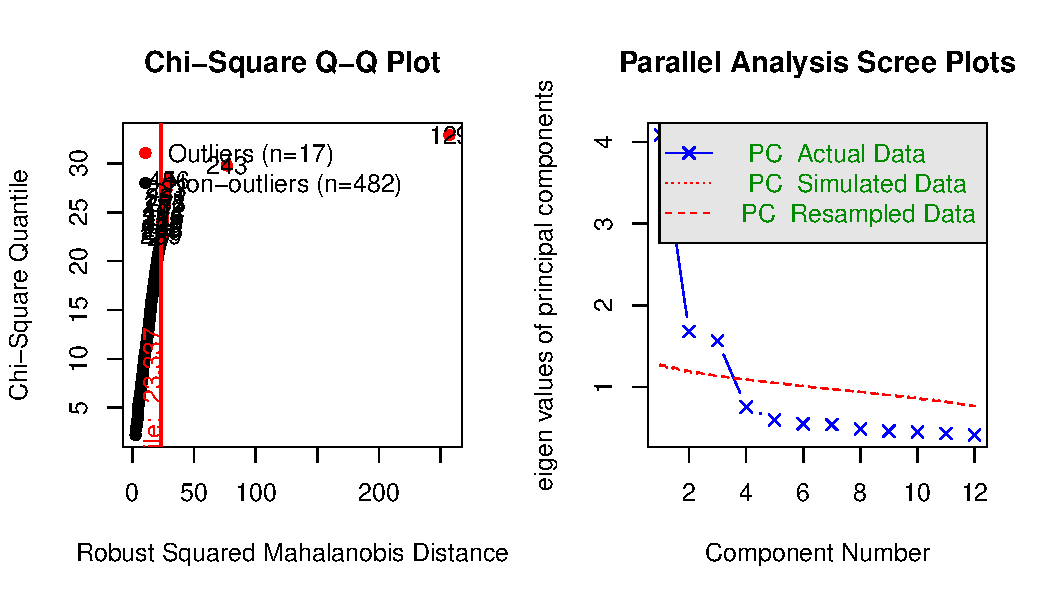
\includegraphics[width=\maxwidth]{figure/unnamed-chunk-10-2} 
\begin{kframe}\begin{verbatim}
## [1] "Case 129 removed. 3 factors remain. This is the 2 round"
\end{verbatim}
\end{kframe}
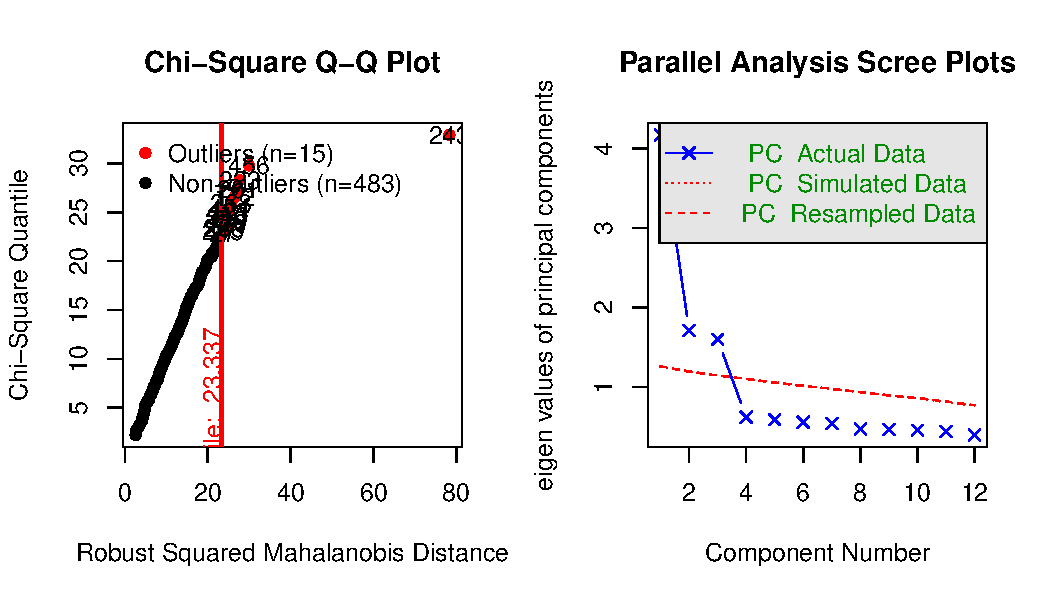
\includegraphics[width=\maxwidth]{figure/unnamed-chunk-10-3} 
\begin{kframe}\begin{verbatim}
## [1] "Case 243 removed. 3 factors remain. This is the 3 round"
\end{verbatim}
\end{kframe}
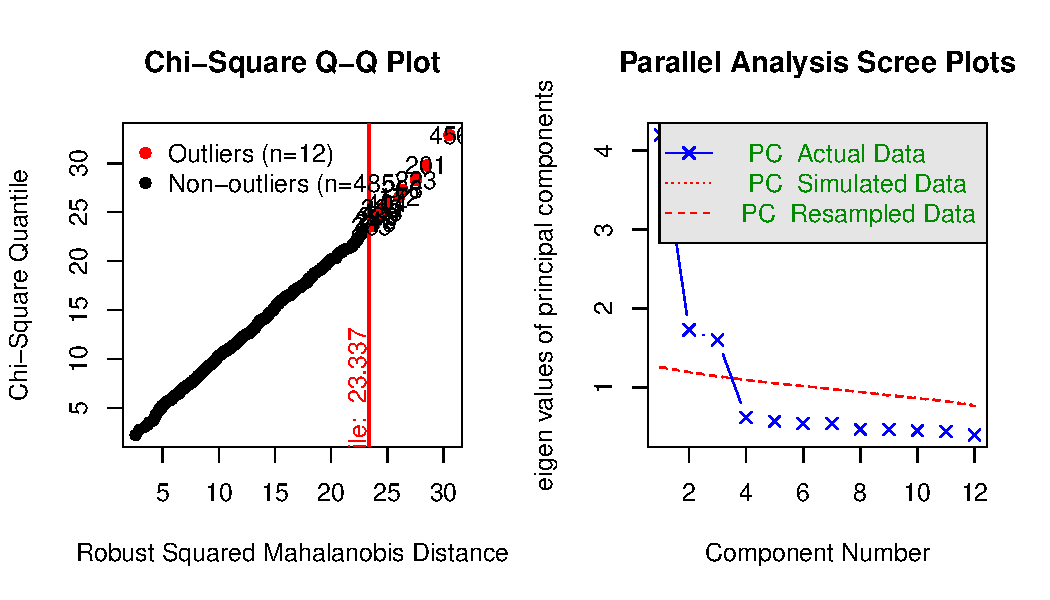
\includegraphics[width=\maxwidth]{figure/unnamed-chunk-10-4} 
\begin{kframe}\begin{verbatim}
## [1] "Case 456 removed. 3 factors remain. This is the 4 round"
\end{verbatim}
\end{kframe}
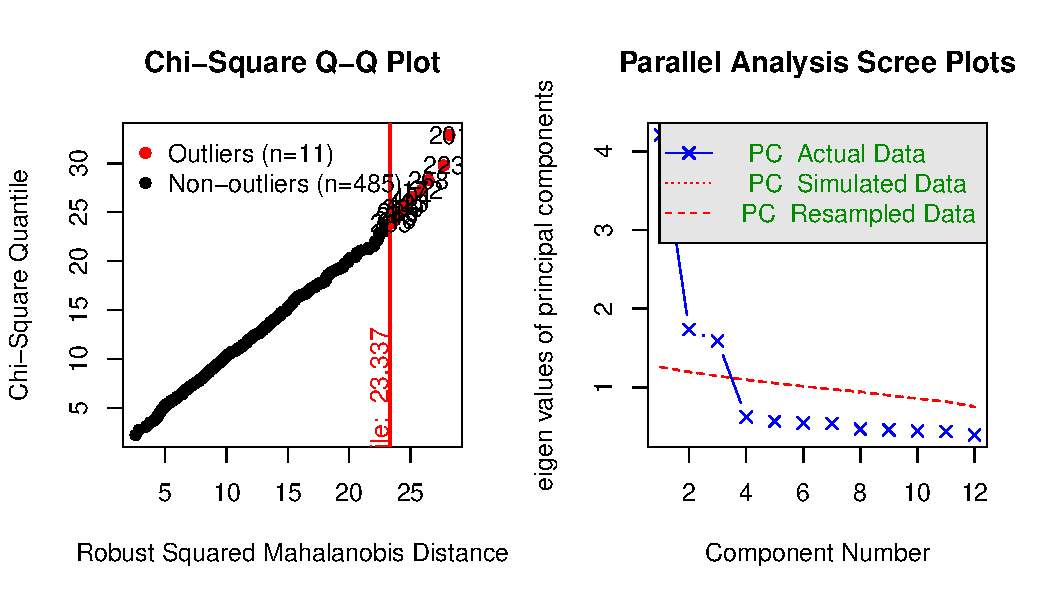
\includegraphics[width=\maxwidth]{figure/unnamed-chunk-10-5} 
\begin{kframe}\begin{verbatim}
## [1] "Case 201 removed. 3 factors remain. This is the 5 round"
\end{verbatim}
\end{kframe}
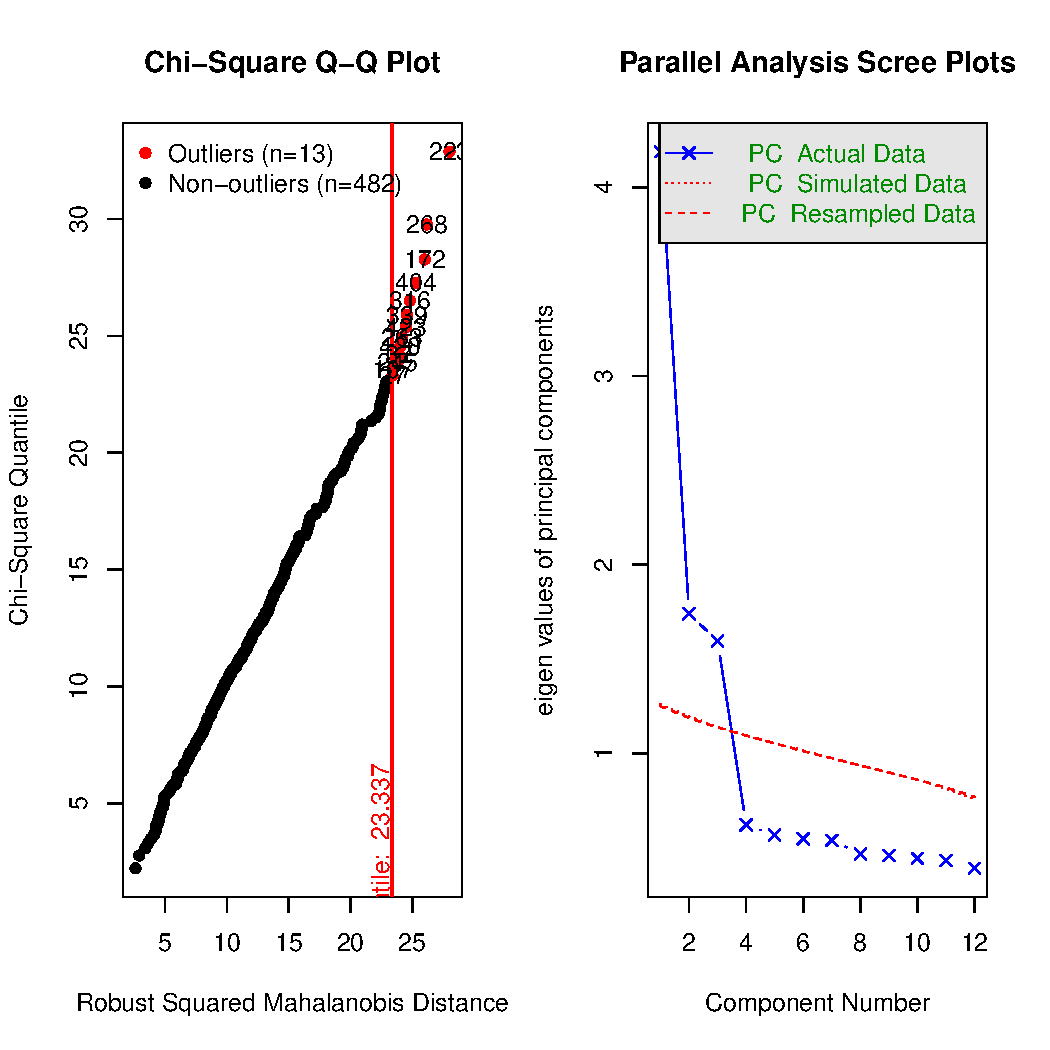
\includegraphics[width=\maxwidth]{figure/unnamed-chunk-10-6} 
\begin{kframe}\begin{verbatim}
## [1] "Case 223 removed. 3 factors remain. This is the 6 round"
\end{verbatim}
\end{kframe}
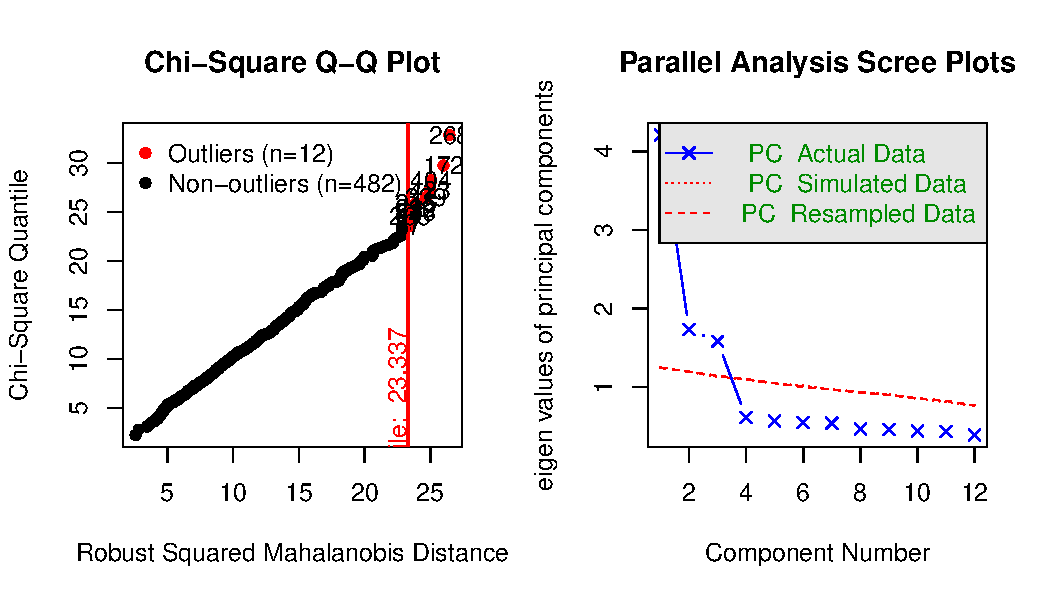
\includegraphics[width=\maxwidth]{figure/unnamed-chunk-10-7} 
\begin{kframe}\begin{verbatim}
## [1] "Case 268 removed. 3 factors remain. This is the 7 round"
\end{verbatim}
\end{kframe}
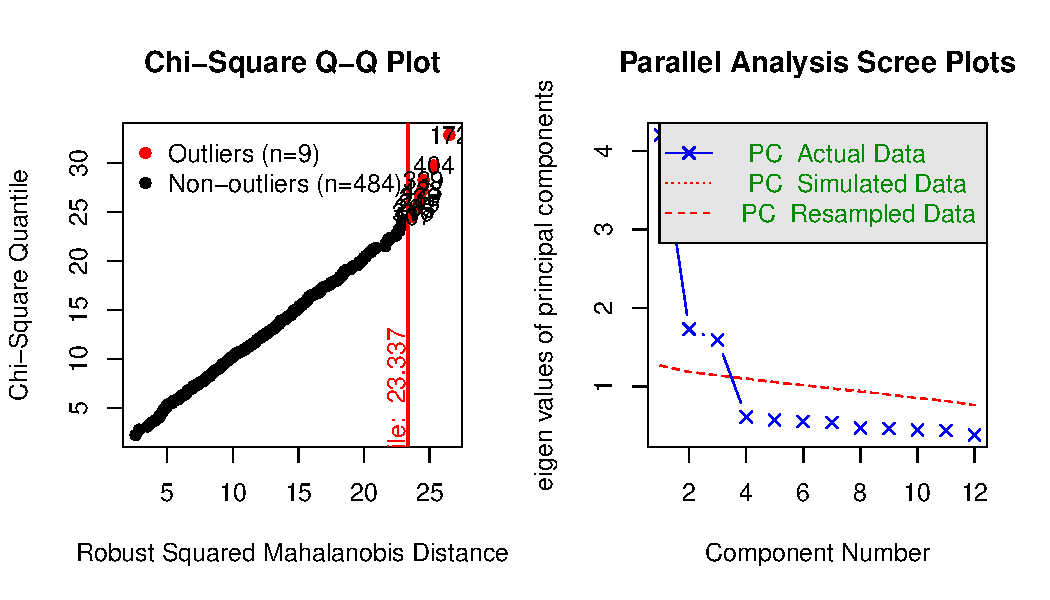
\includegraphics[width=\maxwidth]{figure/unnamed-chunk-10-8} 
\begin{kframe}\begin{verbatim}
## [1] "Case 172 removed. 3 factors remain. This is the 8 round"
\end{verbatim}
\end{kframe}
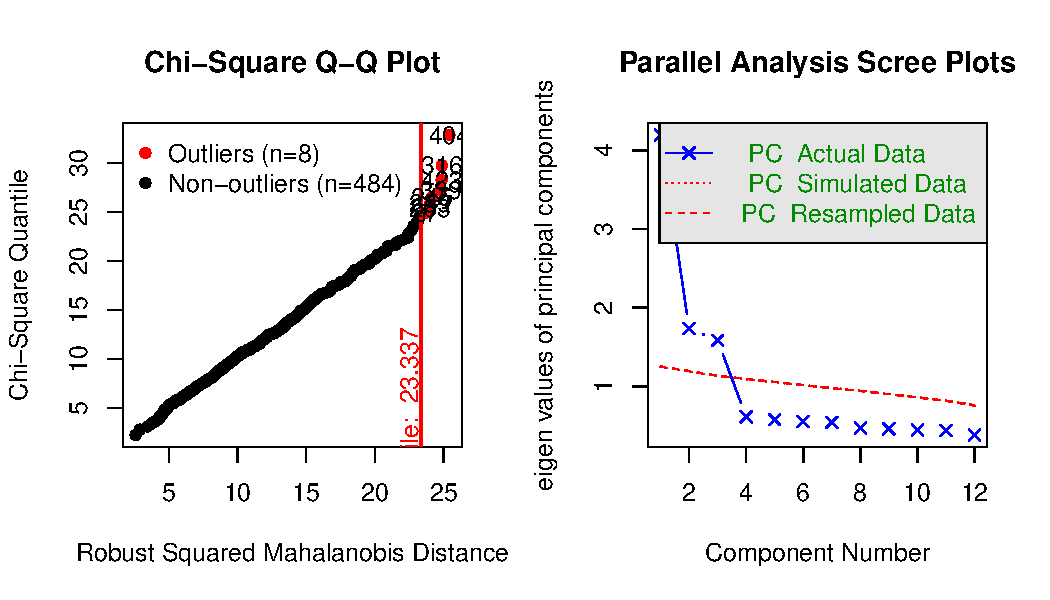
\includegraphics[width=\maxwidth]{figure/unnamed-chunk-10-9} 
\begin{kframe}\begin{verbatim}
## [1] "Case 404 removed. 3 factors remain. This is the 9 round"
\end{verbatim}
\end{kframe}
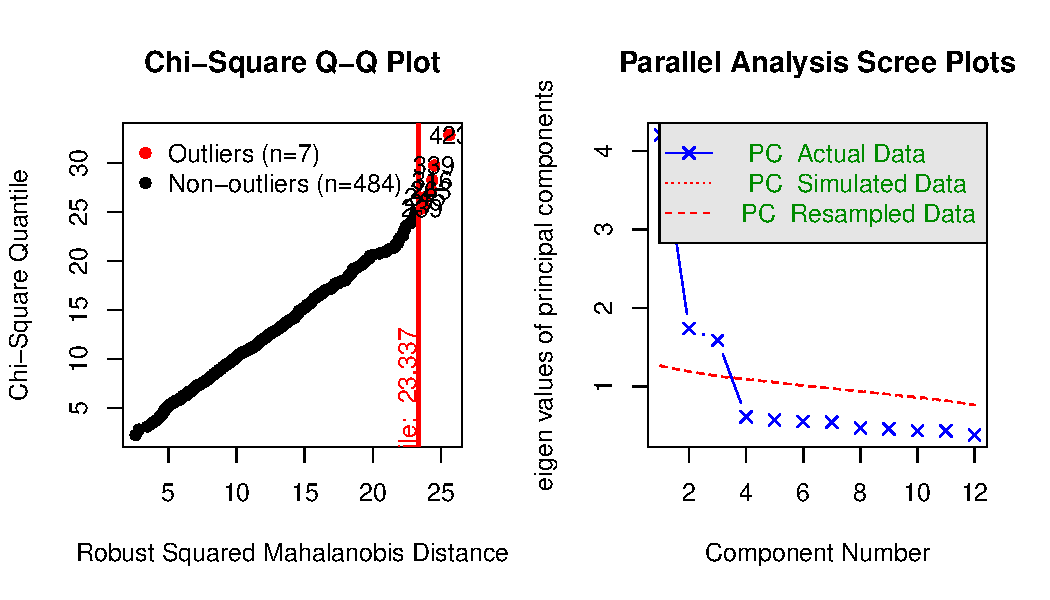
\includegraphics[width=\maxwidth]{figure/unnamed-chunk-10-10} 
\begin{kframe}\begin{verbatim}
## [1] "Case 316 removed. 3 factors remain. This is the 10 round"
\end{verbatim}
\end{kframe}
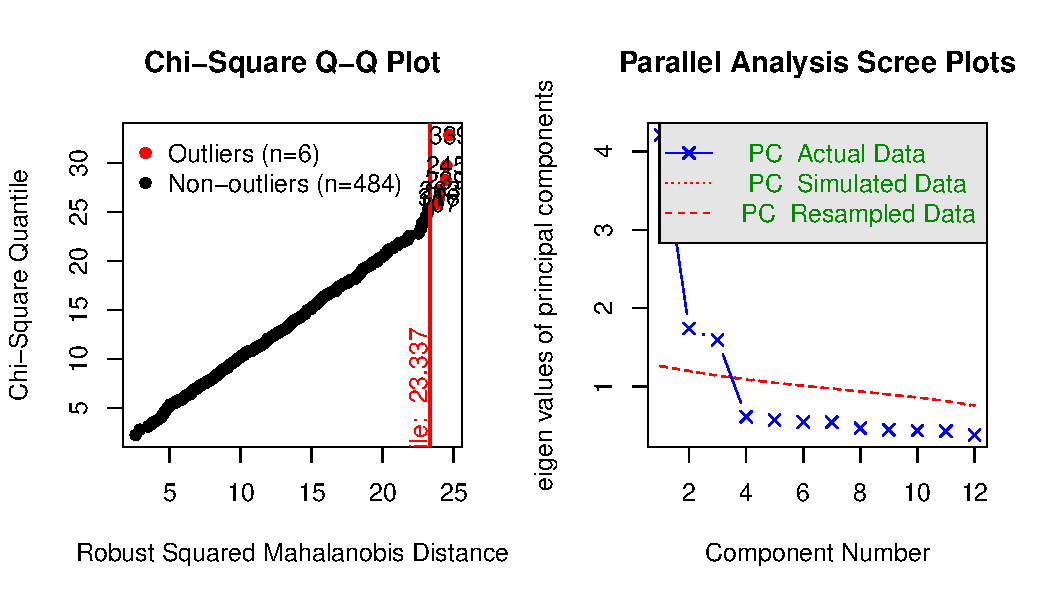
\includegraphics[width=\maxwidth]{figure/unnamed-chunk-10-11} 
\begin{kframe}\begin{verbatim}
## [1] "Case 423 removed. 3 factors remain. This is the 11 round"
\end{verbatim}
\end{kframe}
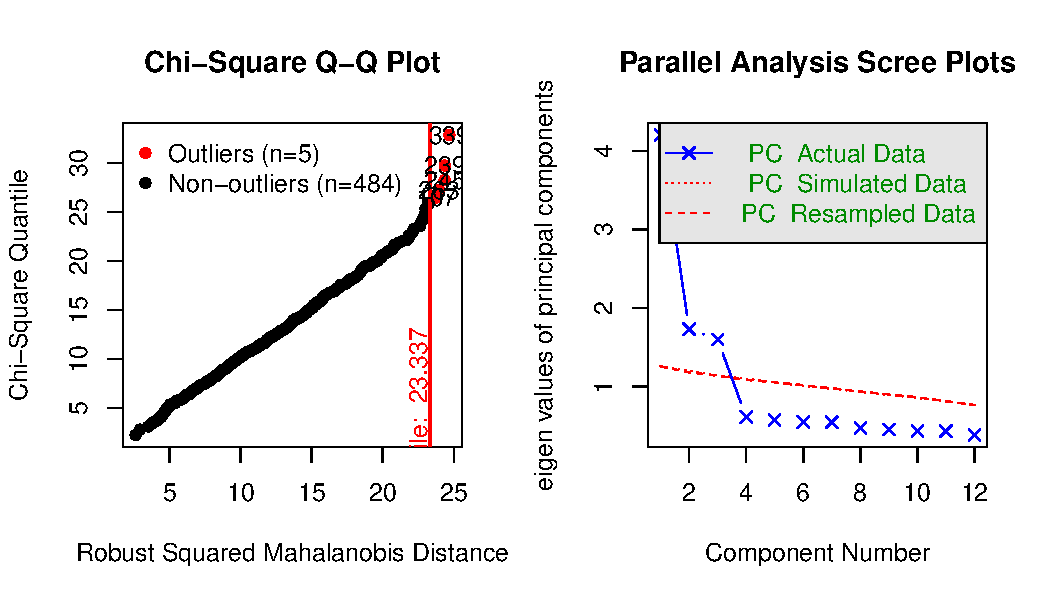
\includegraphics[width=\maxwidth]{figure/unnamed-chunk-10-12} 
\begin{kframe}\begin{verbatim}
## [1] "Case 339 removed. 3 factors remain. This is the 12 round"
\end{verbatim}
\end{kframe}
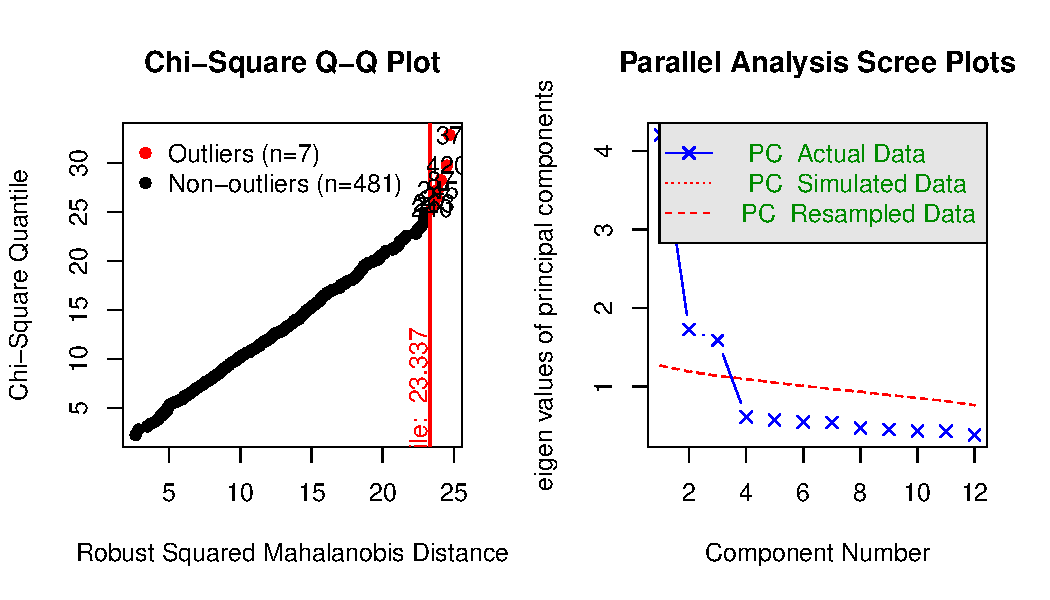
\includegraphics[width=\maxwidth]{figure/unnamed-chunk-10-13} 
\begin{kframe}\begin{verbatim}
## [1] "Case 420 removed. 3 factors remain. This is the 13 round"
\end{verbatim}
\end{kframe}
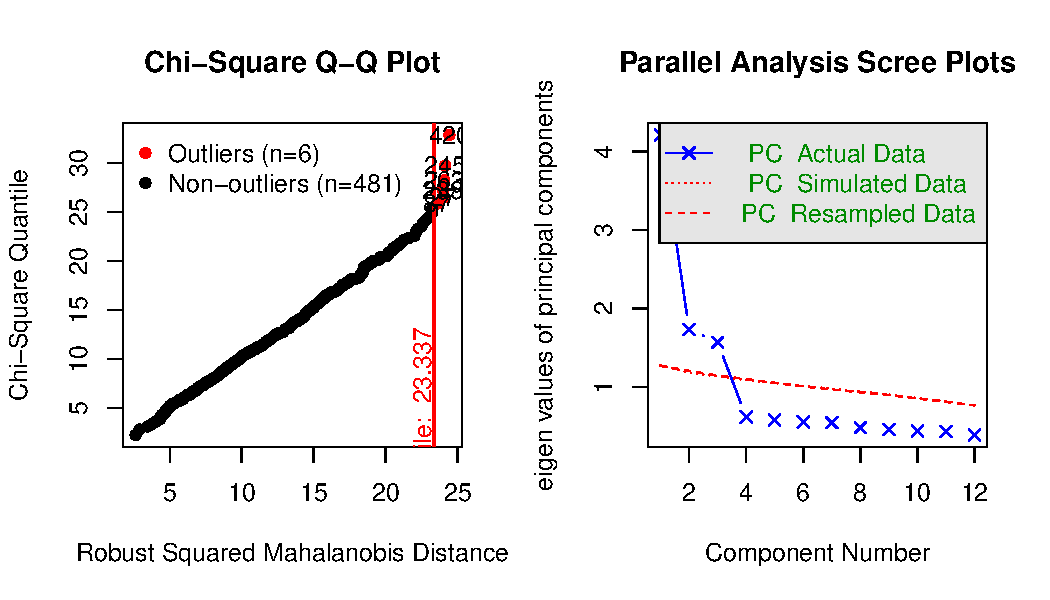
\includegraphics[width=\maxwidth]{figure/unnamed-chunk-10-14} 
\begin{kframe}\begin{verbatim}
## [1] "Case 37 removed. 3 factors remain. This is the 14 round"
\end{verbatim}
\end{kframe}
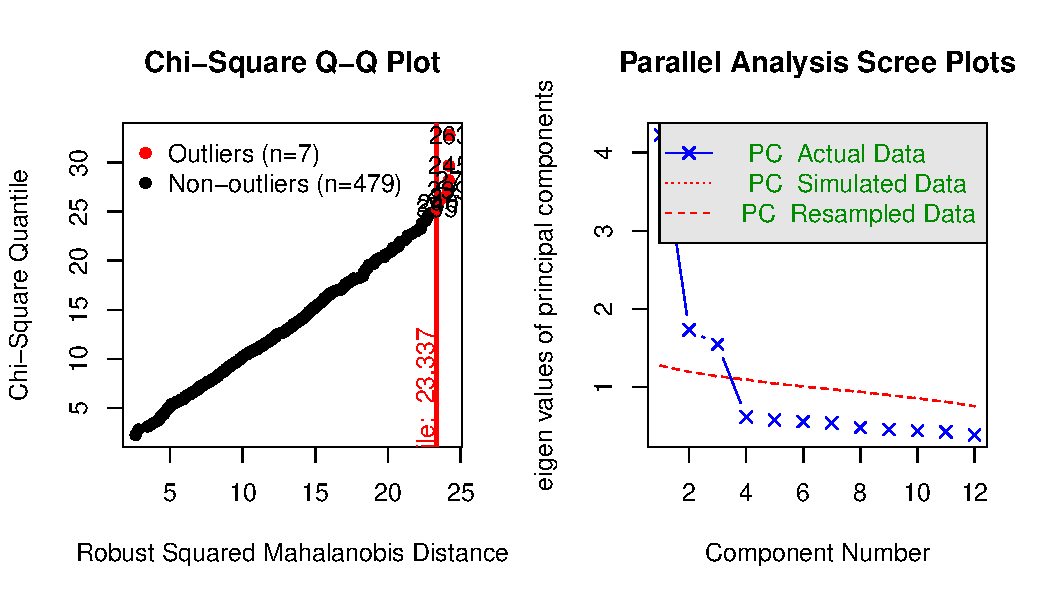
\includegraphics[width=\maxwidth]{figure/unnamed-chunk-10-15} 
\begin{kframe}\begin{verbatim}
## [1] "Case 245 removed. 3 factors remain. This is the 15 round"
\end{verbatim}
\end{kframe}
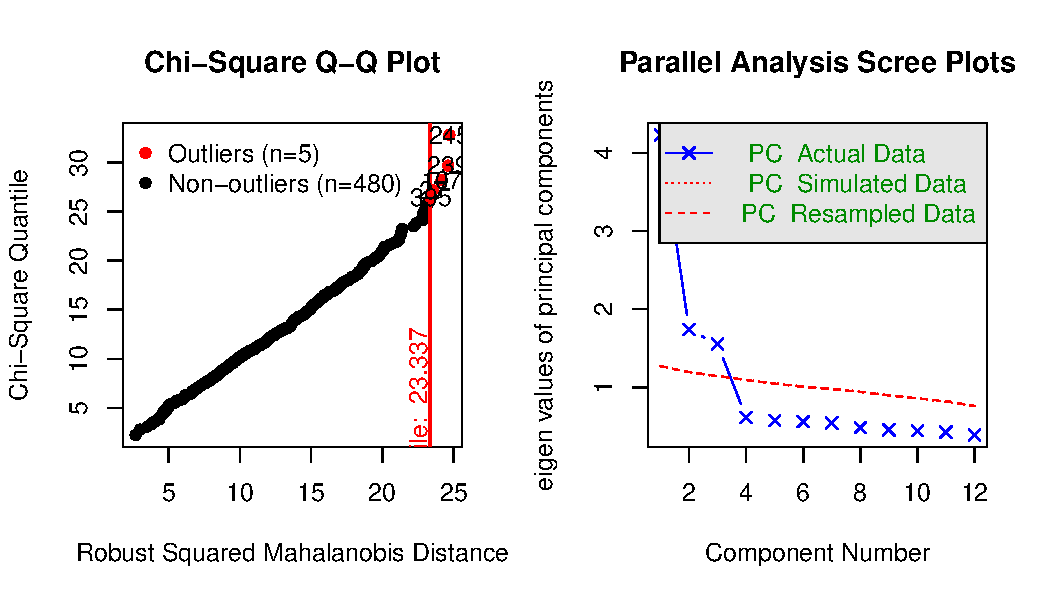
\includegraphics[width=\maxwidth]{figure/unnamed-chunk-10-16} 
\begin{kframe}\begin{verbatim}
## [1] "Case 263 removed. 3 factors remain. This is the 16 round"
\end{verbatim}
\end{kframe}
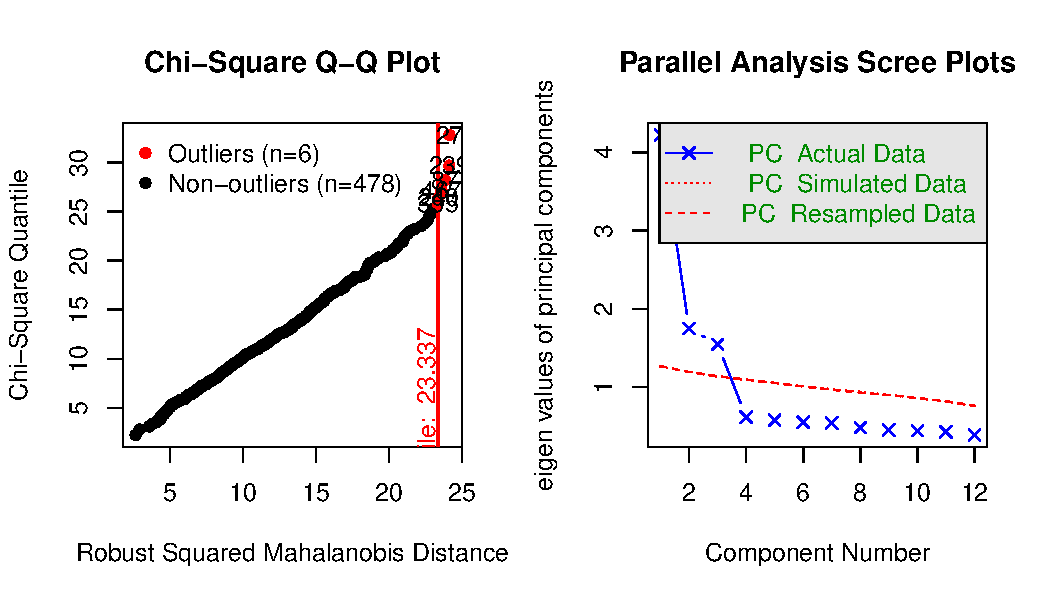
\includegraphics[width=\maxwidth]{figure/unnamed-chunk-10-17} 
\begin{kframe}\begin{verbatim}
## [1] "Case 239 removed. 3 factors remain. This is the 17 round"
\end{verbatim}
\end{kframe}
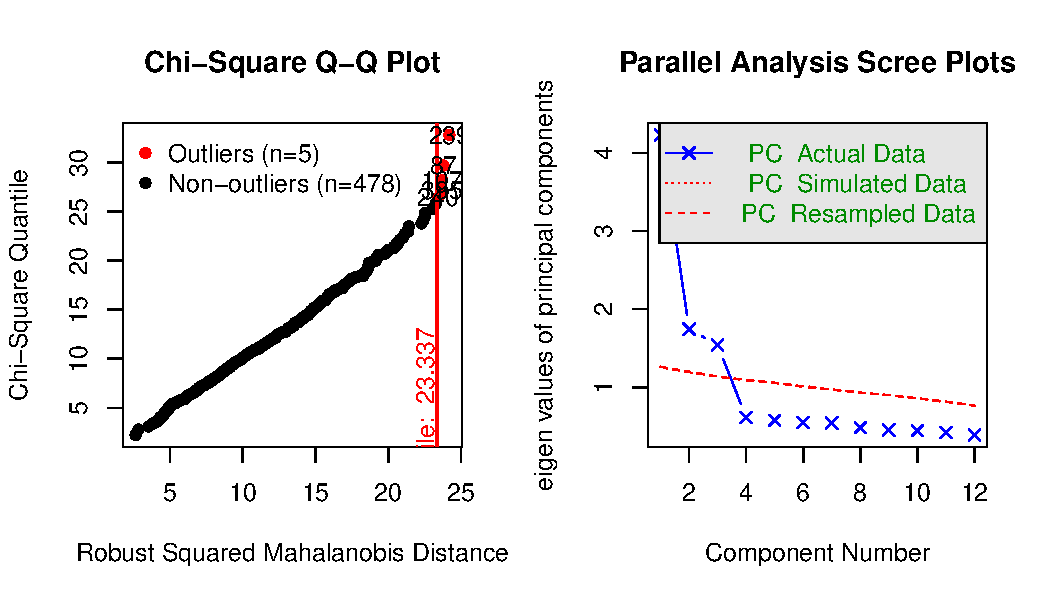
\includegraphics[width=\maxwidth]{figure/unnamed-chunk-10-18} 
\begin{kframe}\begin{verbatim}
## [1] "Case 27 removed. 3 factors remain. This is the 18 round"
\end{verbatim}
\end{kframe}
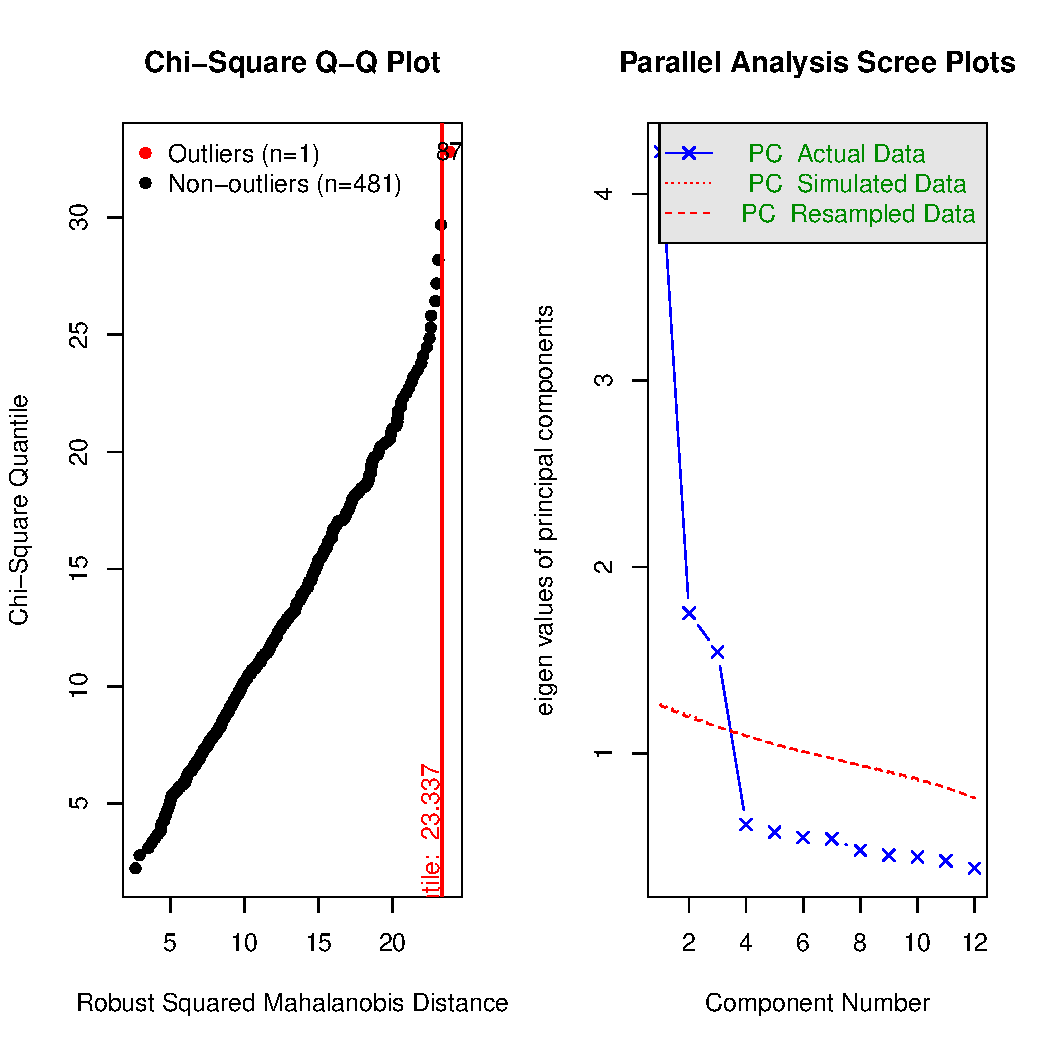
\includegraphics[width=\maxwidth]{figure/unnamed-chunk-10-19} 
\begin{kframe}\begin{verbatim}
## [1] "Case 87 removed. 3 factors remain. This is the 19 round"
\end{verbatim}
\end{kframe}
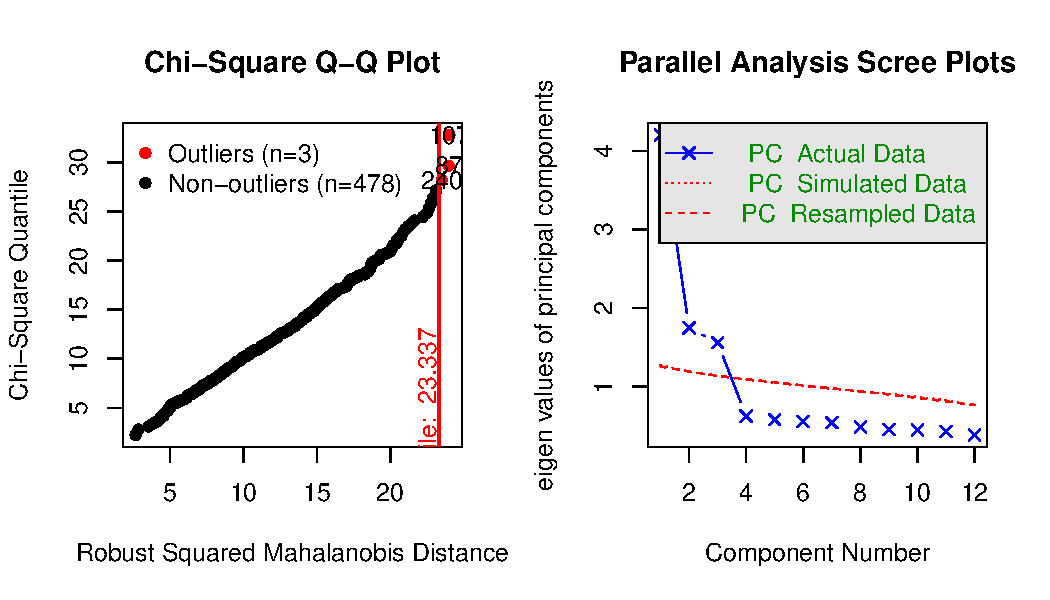
\includegraphics[width=\maxwidth]{figure/unnamed-chunk-10-20} 
\begin{kframe}\begin{verbatim}
## [1] "Case 107 removed. 3 factors remain. This is the 20 round"
\end{verbatim}
\end{kframe}
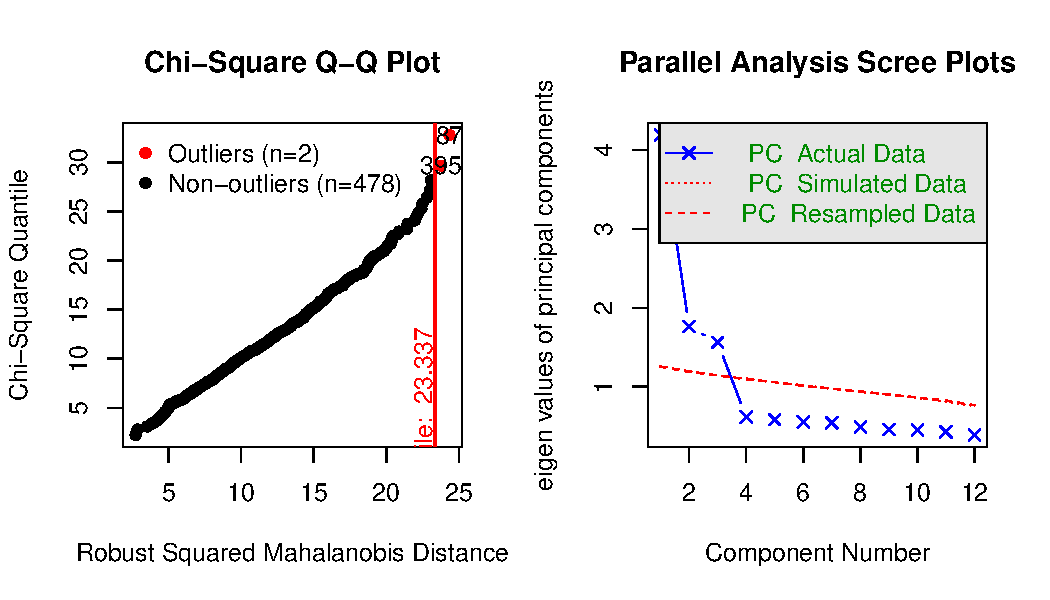
\includegraphics[width=\maxwidth]{figure/unnamed-chunk-10-21} 
\begin{kframe}\begin{verbatim}
## [1] "Case 240 removed. 3 factors remain. This is the 21 round"
\end{verbatim}
\end{kframe}
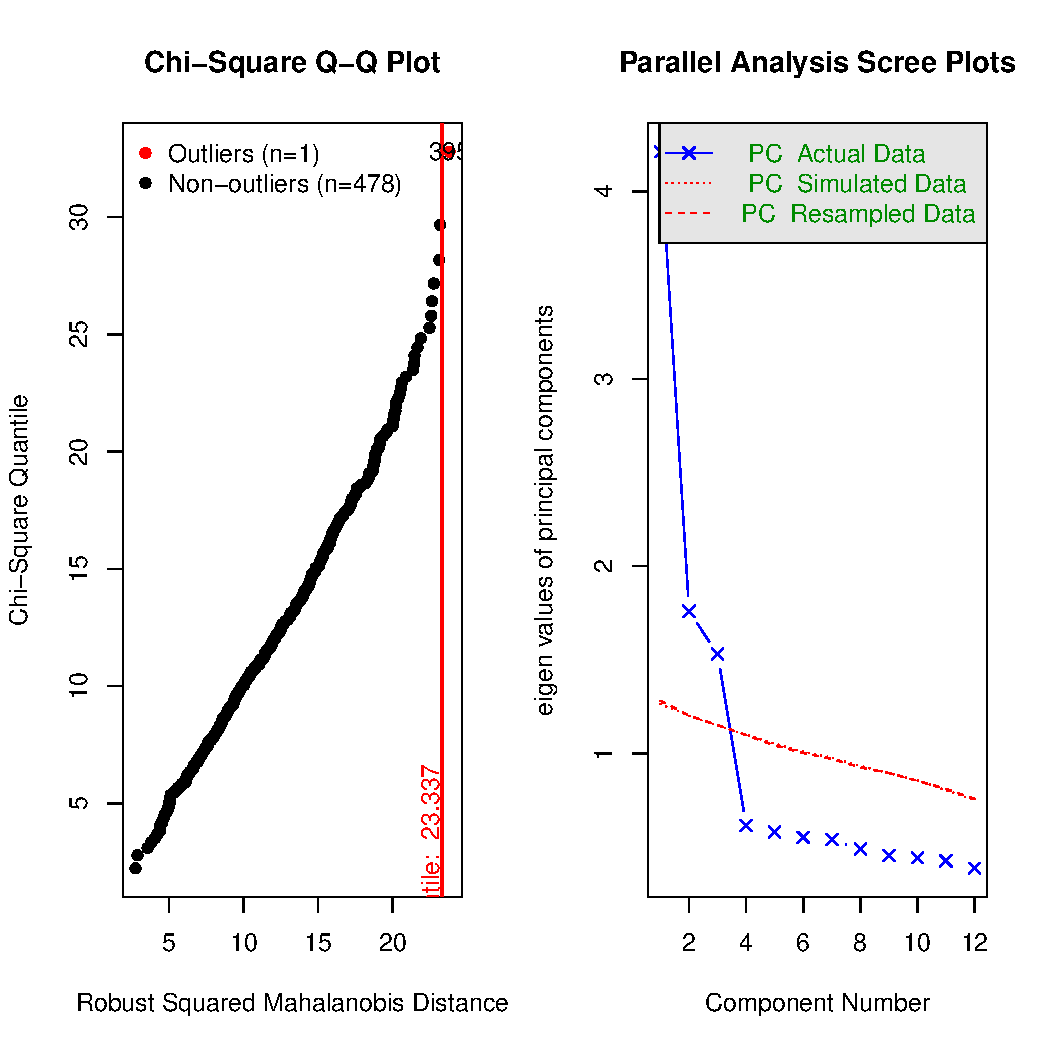
\includegraphics[width=\maxwidth]{figure/unnamed-chunk-10-22} 
\begin{kframe}\begin{verbatim}
## [1] "Case 395 removed. 3 factors remain. This is the 22 round"
\end{verbatim}
\end{kframe}
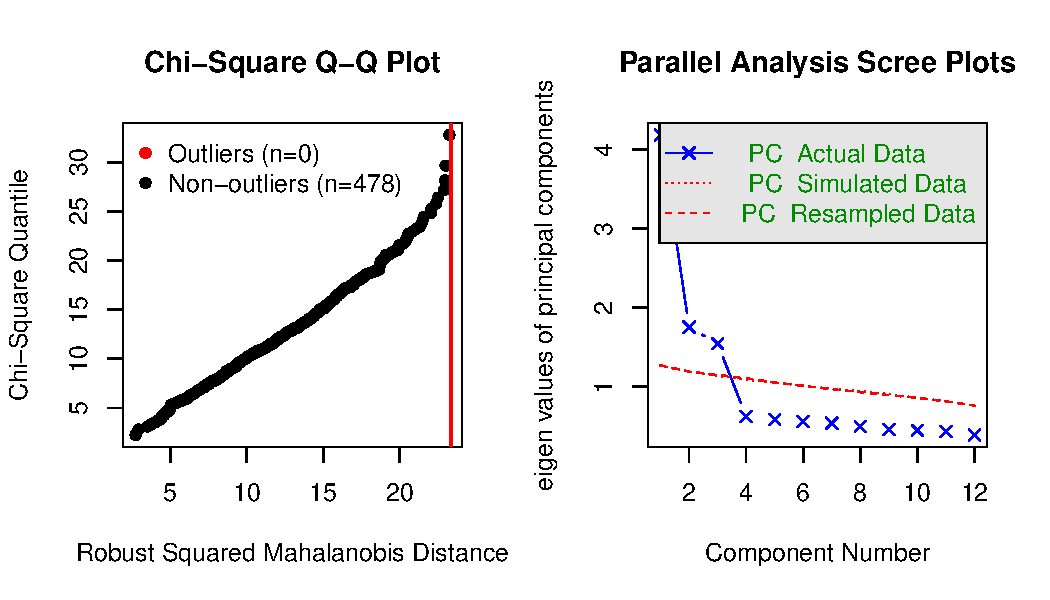
\includegraphics[width=\maxwidth]{figure/unnamed-chunk-10-23} 
\begin{kframe}\begin{verbatim}
## [1] "Case NA removed. 3 factors remain. This is the 23 round"
\end{verbatim}
\end{kframe}
\end{knitrout}

In total, using the mardia test, it took 23 rounds to remove the following outliers: cases .

Our conclusions do not change. We would still extract 3 components.




\end{document}
